\documentclass[aspectratio=169]{beamer}

\usepackage[utf8]{inputenc} % codificacao de caracteres
\usepackage[T1]{fontenc}    % codificacao de fontes
\usepackage[brazil]{babel}  % idioma

\usepackage{setspace}
\usepackage{listings}		% códigos
\usepackage{parcolumns}
\usepackage{color}

\usepackage{hyperref}		% hyperlink

\usepackage{graphicx}		% imagens
\usepackage{caption}
\usepackage{subcaption}

\definecolor{mygreen}{rgb}{0,0.6,0}
\definecolor{mygray}{rgb}{0.5,0.5,0.5}
\definecolor{mymauve}{rgb}{0.58,0,0.82}

\lstdefinestyle{scriptstyle}{
  belowcaptionskip=1\baselineskip,
  breaklines=true,
  frame=L,
  language=Python,
  xleftmargin=\parindent,
  showstringspaces=false,
  basicstyle=\footnotesize\ttfamily,
  keywordstyle=\bfseries\color{green!40!black},
  commentstyle=\itshape\color{purple!40!black},
  identifierstyle=\color{blue},
  stringstyle=\color{orange},
  numbers=left,
  numbersep=10pt,
  tabsize=4,
  firstline=1,
  texcl=true,
  escapeinside={//}{\^^M}
}

\lstdefinestyle{ipythonstyle}{
  belowcaptionskip=1\baselineskip,
  breaklines=true,
  frame=L,
  language=Python,
  xleftmargin=\parindent,
  showstringspaces=false,
  basicstyle=\footnotesize\ttfamily,
  keywordstyle=\bfseries\color{green!40!black},
  commentstyle=\itshape\color{purple!40!black},
  identifierstyle=\color{blue},
  stringstyle=\color{orange},
  texcl=true,
  escapeinside={//}{\^^M}
}

\lstset{escapechar=@,style=ipythonstyle, texcl=true, escapeinside={//}{\^^M}}

\setbeamertemplate{footline}[frame number]
\usetheme{metropolis}         % tema
\usecolortheme{orchid}      % cores
\usefonttheme[onlymath]{serif} % fonte modo matematico

% Titulo
\title{Python, o que é e porque usar}
\author[Gustavo Santos]{Gustavo Fernandes dos Santos \\
\texttt{gfdsantos@inf.ufpel.edu.br}}
\institute{UFPEL - Universidade Federal de Pelotas}

\date{\today}

%---------------------------------------------------------

\begin{document}

%-------------- TITULO --------------
\begin{frame}
  \titlepage
\end{frame}

\begin{frame}{Sobre o autor}
    \frametitle{whoami}
    \begin{itemize}
        \item Programador Python há 6 anos
        \item Pregador do software livre há 4 anos
        \item Curioso por natureza
        \item Estudante de Engenharia de Computação
    \end{itemize}
\end{frame}

\begin{frame}
	\frametitle{Para quem é esta apresentação?}
	Para mim! Eu fiz essa apresentação pra mim. Minha memória não é boa, nunca foi boa
o suficiente para tudo que eu quero/preciso saber. Trabalho com muitas linguagens hoje.
Na faculdade preciso programar muito bem em C, Java e VHDL. Também desenvolvo aplicativos
para Android, preciso manter o ecossistema em mente. Mantenho o meu servidor local escrito
em Scala. Também já programei em Fortran, Haskell e Erlang, puramente para conhecer
melhor estas linguagens e os paradigmas que implementam. Fazer essa apresentação foi um modo
que encontrei para lembrar rapidamente de alguma questão básica sobre Python.

	Esta apresentação é a primeira de uma série de apresentações sobre as demais linguagens
e frameworks que conheço.
\end{frame}

%-------------- INDICE --------------
\begin{frame}{Indice}
    \tableofcontents
\end{frame}

%---------------------------------------------------------

\section{Historinha do Python}

\begin{frame}
    \frametitle{O que é Python?}
    Python é uma linguagem de programação de propósito geral. É uma linguagem de
script, logo obedece às regras de linguagens de script. Python é,
muitas vezes, definida como uma \textbf{linguagem de script orientada a objetos}. A
definição anterior acaba limitando o escopo atual do Python, que pode ser definido
mais precisamente como uma \textbf{linguagem de programação de propósito geral, que
suporta os paradigmas de programação procedural, funcional e orientado a objetos}.
\end{frame}

\begin{frame}
    \frametitle{Porque as Pessoas Usam Python?}
    Esta é uma das primeiras questões que aparecem quando as pessoas pensam em
usar Python. Existem tantas linguagens de programação por aí hoje que escolher uma
linguagem específica para um determinado projeto torna-se uma tarefa difícil.

    Mas não há regras. É uma questão pessoal. Mas há uma série de fatores que
acabam chamando a atenção dos desenvolvedores para a linguagem da cobrinha.
\end{frame}

\begin{frame}
    \frametitle{Porque as Pessoas Usam Python?}
    \begin{itemize}
        \item \textbf{Produtividade.} Python é uma linguagem que proporciona que o
mesmo que seria feito em alguma linguagem compilada e estaticamente tipada faria, mas com
muito mais rapidez, reduzindo drasticamente o tempo de desenvolvimento do projeto. O
código em Python é geralemnte 3 ou 5 vezes menor que o código equivalente em C++. Programas
em Python rodam imediatamente após serem escritos, não necessitando de nenhum processo de
compilação, ligação ou montagem.
        \item \textbf{Portabilidade.} A maioria dos programas escritos em Python rodam
na maioria dos sistemas operacionais para computadores. Um código pode ser totalmente
portável entre Linux, Mac e Windows, se não utilizar ferramentas específicas destes
sistemas operacionais. Python é interpretado, logo um sistema apenas necessita implementar
o interpretador para rodar o código em Python. Existem
também diversas bibliotecas de interface de usuário portáveis. Característica que permite que
um programa tenha a mesma interface independente de onde seja executado.
    \end{itemize}
\end{frame}

\begin{frame}
    \frametitle{Porque as pessoas usam Python?}
    \begin{itemize}
        \item \textbf{Suporte.} Python vem por padrão com uma coleção incrível de baterias.
Contudo há uma infinidade de bibliotecas para as distribuições de Python, como bibliotecas
de deep leaning - \textit{Tensorflow}, \textit{Theano} e etc; visão computacional,
tendo como destaque a biblioteca \textit{OpenCV}. Python também também tem bibliotecas para
computação numérica, como o \textit{NumPy}, análise de dados com o \textit{Pandas},
desenvolvimento web com \textit{Django}, \textit{Flask} e muitas outras.
        \item \textbf{Integração.} Python consegue facilmente se integrar com partes
de alguma outra aplicação, como invocar códigos C e C++ e ser invocado por programas escritos
em C ou C++. Pode se integrar com componentes Java e .NET. Python não é uma ferramenta
singular, Python pode conviver facilmente com outros ecossistemas.
    \end{itemize}
\end{frame}

\begin{frame}
    \frametitle{Existe alguma parte ruim?}
    Python é uma linguagem de script, é interpretada. O fato de Python ser interpretado
implica que nem sempre os programas em Python irão rodar com a mesma velocidade que programas
equivalentes escritos em C/C++. Isto é relativamente raro hoje, mas ainda acontece.

    A implementação em Python padrão hoje (3.5.2) traduz o código fonte para um código
intermediário. O código intermediário - bytecode - é interpretado pela máquina virtual. Como
o código em bytecode é interpretado, em vez de rodar diretamente no processador, há perdas
de performance se comparados com código objeto gerado pelo gcc, por exemplo.
\end{frame}

\begin{frame}[fragile]
    \begin{lstlisting}
In [1]: def mult(x, y):
   ...:     z = x * y
   ...:     return z
   ...:

In [2]: from dis import dis

In [3]: dis(mult)
  2           0 LOAD_FAST                0 (x)
              3 LOAD_FAST                1 (y)
              6 BINARY_MULTIPLY
              7 STORE_FAST               2 (z)

  3          10 LOAD_FAST                2 (z)
             13 RETURN_VALUE
    \end{lstlisting}
\end{frame}

\begin{frame}
    \frametitle{Existe alguma parte ruim?}
    O tempo de execução sempre irá depender do quanto você está disposto a abrir mão
em prol das outras características boas do Python. No fim das contas, você irá decidir
se vale mais a pena abrir mão de alguns milissegundos do tempo de execução ou dispender
mais tempo com o desenvolvimento e manutenção da aplicação em alguma outra linguagem
compilada, como C/C++.

    Considerando a evolução das CPUs e a velocidade com que os dados são processados
atualmente, na grande maioria dos casos, optar por uma linguagem como Python torna-se
natural e seguro. Ainda mais considerando que é possível escrever as partes mais críticas
do software em C/C++ e integrar com sua aplicação em Python.
\end{frame}

\begin{frame}
    \frametitle{Quem usa Python?}
    Python dispõe de uma grande base de usuários e uma comunidade bastante ativa. Há vários
anos diferentes ranks de uso de linguagens de programação citam Python como uma das 5
linguagens mais usadas.

    \begin{itemize}
        \item \textbf{Google.} Google usa largamente Python na sua ferramenta de indexação -
 Google Search. A empresa também usa Python para desenvolver seus sistemas de inteligencia
artificial.
        \item \textbf{Youtube.} Como um serviço do Google, o Youtube também usa largamente
Python por baixo dos panos.
        \item \textbf{Dropbox.} O cliente do Dropbox para desktops é escrito em Python.
        \item \textbf{Pixar.} A Pixar (Toy Story) usa Python na produção de seus filmes de
animação.
        \item \textbf{NSA.} A agência americana usa Python para análise e criptografia dos
dados.
        \item \textbf{Netflix.} A Netflix usa Python na sua infraestrutura de software.
    \end{itemize}
\end{frame}

\begin{frame}
    \frametitle{O poder do Python}
    Python está entre uma linguagem de script e linguagem de desenvolvimento de sistemas.
Python contém toda a facilidade e simplicidade de linguagens de script (como Perl, Ruby e
Scheme) e também ferramentas poderosas de engenharia de software, encontradas tipicamente
em linguagens compiladas (como Java e C++).

    \begin{itemize}
        \item \textbf{Tipagem dinâmica.} Nomes (variáveis) em Python são apenas referências
a objetos, objetos não ficam atrelados a um tipo específico de dado, são mutáveis.
        \item \textbf{Gerenciamento de memória automático.} Python contém um coletor de
lixo embutido na máquina virtual. Além disso, Python consegue alocar automaticamente
objetos. O desenvolvedor não precisa se preocupar com problemas de baixo nível, a máquina
virtual trata todos estes problemas automaticamente.
    \end{itemize}
\end{frame}

\begin{frame}
    \frametitle{O poder do Python}
    \begin{itemize}
        \item \textbf{Estruturas de dados incluídas.} Python vêm com as estruturas de
dados mais utilizadas como listas, dicionários e strings como parte da linguagem.
        \item \textbf{Programação escalável.} Python contém ferramentas para desenvolvimento
de sistemas de larga escala, como modulos, classes e excessões.
        \item \textbf{Ferramentas de terceiros.} Python é livre e aberto. Desenvolvedores
são encorajados a contribuír com ferramentas. Você consegue encontrar ferramentas para
acesso a bancos de dados, programação numérica, desenvolvimento de sistemas inteligentes,
desenvolvimento web e muito mais.
    \end{itemize}
\end{frame}

%---------------------------------------------------------

\section{Ferramentas Interessantes}

\begin{frame}
    \frametitle{CPython}
    CPython é a distribuição padrão do Python. O interpretador da linguagem é escrito
em ANSI C, o que dá a esta implementação maior poder de portabilidade. O desenvolvimento
é encabeçado pelo criador da linguagem Python:
Guido van Rossum e pelo grupo principal de desenvolvimento da linguagem. A distribuição padrão vêm com
um tradutor de código fonte para bytecode e com uma máquina virtual, chamada de \textbf{Python Virtual Machine}.

	Além do CPython, existem outras implementações conhecidas da linguagem, como
\textbf{JPython}, \textbf{IronPython}, \textbf{Stackless} e \textbf{PyPy}.
\end{frame}

\begin{frame}[fragile]
    \frametitle{CPython}
	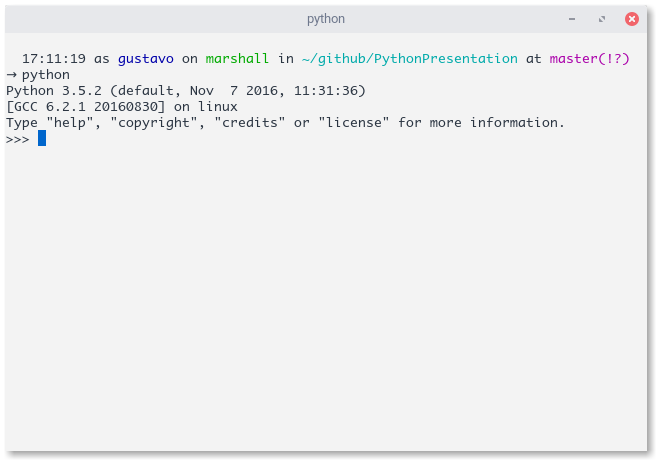
\includegraphics[scale=0.45]{python_imgs/console_python}
\end{frame}

\begin{frame}
    \frametitle{IPython}
    O IPython pode ser visto como o REPL padrão do Python, com esteroides. O objetivo do IPython é
disponibilizar um ambiente exploratório de computação interativa.
    Esta apresentação foi construída quase que em sua totalidade utilizando o IPython para
debug dos trechos de códigos mostrados ao longo da apresentação.
\end{frame}

\begin{frame}[fragile]
    \frametitle{IPython}
	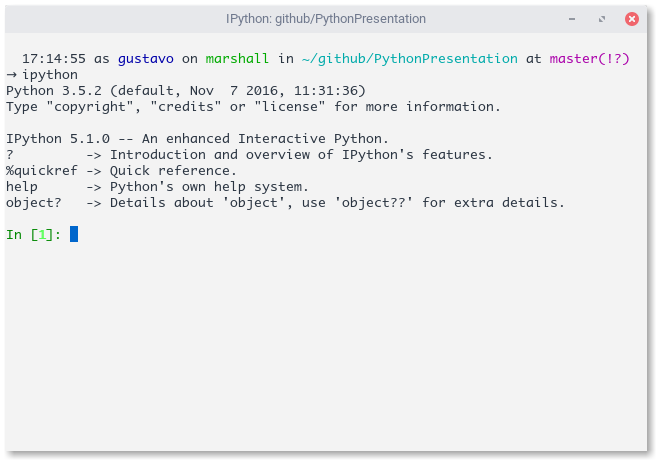
\includegraphics[scale=0.45]{python_imgs/console_ipython}
\end{frame}

\begin{frame}
    \frametitle{PyPy}
    PyPy é uma implementação alternativa do CPython, focada na performance. A grande diferença
entre o PyPy e o CPython padrão é que o PyPy vêm com um compilador JIT - Just In Time. O
compilador JIT é acoplado ao PVM como uma extensão, traduzindo partes do código fonte, apenas
quando necessário. O PyPy consegue executar programas longos escritos em Python, entre 3-5 vezes
mais rápido que a implementação padrão - CPython.
\end{frame}

\begin{frame}[fragile]
    \frametitle{PyPy}
	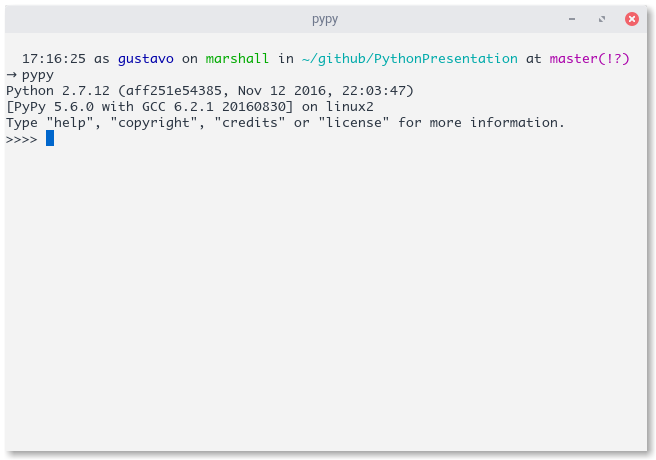
\includegraphics[scale=0.45]{python_imgs/console_pypy}
\end{frame}

%---------------------------------------------------------

\section{A Linguagem}

\begin{frame}[fragile]
	\frametitle{Tipos básicos de dados}
	\begin{lstlisting}
In [1]: type(2**512)
Out[1]: int

In [2]: type([1, 2, 3])
Out[2]: list

In [3]: type((1, 2, 3))
Out[3]: tuple

In [4]: type({1: "Marie", 2: "Maribel", 3: "Meggie", 4: "Elisa"})
Out[4]: dict

In [5]: type("oi, tudo bem?")
Out[5]: str
	\end{lstlisting}
\end{frame}

\begin{frame}[fragile]
	\frametitle{Tipos básicos de dados}
	\begin{lstlisting}
In [6]: type(lambda x: x + x)
Out[6]: function

In [7]: type(False)
Out[7]: bool

In [8]: type(1.23e-4)
Out[8]: float

In [9]: type(range(10))
Out[9]: range

In [10]: type(enumerate([1, 2, 3]))
Out[10]: enumerate
	\end{lstlisting}
\end{frame}

\begin{frame}[fragile]
	\frametitle{Operações aritméticas}

	\noindent\begin{minipage}{.5\textwidth}
		\begin{lstlisting}
In [29]: 1 + 2
Out[29]: 3

In [30]: 1 * 2
Out[30]: 2

In [31]: 1 / 2
Out[31]: 0.5

In [32]: 1 ** 2
Out[32]: 1
		\end{lstlisting}
		\end{minipage}\hfill
		\begin{minipage}{.45\textwidth}
		\begin{lstlisting}
In [33]: 1 >> 2
Out[33]: 0

In [34]: 1 << 2
Out[34]: 4

In [35]: 1 % 2
Out[35]: 1
		\end{lstlisting}
	\end{minipage}
\end{frame}

\begin{frame}[fragile]
	\frametitle{Referências a objetos}
	Python não possui variáveis, em vez disto, possui referências a objetos, que são
conhecidos como nomes.

	\begin{lstlisting}
In [11]: g = lambda x: x*x + 2*x

In [12]: a = 4

In [13]: b = 5

In [14]: l = [1, 2, 3, 4, 5]

In [15]: t = (1, 2, 3, 4, 5)

In [16]: d = {0: "oi", "tudo": 1, 2: "bem?"}
	\end{lstlisting}
\end{frame}

\begin{frame}[fragile]
	\frametitle{Operador de identificação}
	\begin{lstlisting}
In [36]: n1 = 4

In [37]: n2 = 4

In [38]: n1 == n2
Out[38]: True

In [39]: n1 is n2
Out[39]: True

In [40]: n3 = 5

In [41]: n1 is n3
Out[41]: False
	\end{lstlisting}
\end{frame}

\begin{frame}[fragile]
	\frametitle{Operador de identificação}
	\begin{lstlisting}
In [42]: l1 = [1, 2, 3, 4]

In [43]: l2 = [1, 2, 3, 4]

In [44]: l1 == l2
Out[44]: True

In [45]: l1 is l2
Out[45]: False

In [46]: l1 = l2

In [47]: l1 is l2
Out[47]: True
	\end{lstlisting}
\end{frame}


\begin{frame}[fragile]
	\frametitle{Operações lógicas}
	\begin{lstlisting}
In [52]: True or False
Out[52]: True

In [53]: True and False
Out[53]: False

In [54]: True or False and True
Out[54]: True

In [55]: True and False and True
Out[55]: False
	\end{lstlisting}
\end{frame}


\begin{frame}[fragile]
	\frametitle{Operadores de comparação}
	\begin{lstlisting}
In [56]: x = 1; y = 2

In [57]: x == y
Out[57]: False

In [58]: x != y
Out[58]: True

In [59]: x < y
Out[59]: True

In [60]: x >= y
Out[60]: False

In [61]: 0 < x < y
Out[61]: True
	\end{lstlisting}
\end{frame}


\begin{frame}[fragile]
	\frametitle{Operadores de comparação}
	\begin{lstlisting}
In [62]: t = ("gustavo", 1994, [1, 2, 3], lambda n: n < 1)

In [63]: 1994 in t
Out[63]: True

In [65]: (lambda n: n < 1) in t
Out[65]: False

In [66]: [1, 2, 3] in t
Out[66]: True

In [67]: "gustavo" in t
Out[67]: True
	\end{lstlisting}
\end{frame}


\begin{frame}[fragile]
	\frametitle{Fluxo de controle}
	\begin{lstlisting}
if <expres_booleana>:
	<comandos>
elif <expres_booleana>:
	<comandos>
else:
	<comandos>

In [69]: if 3 > 1:
    ...:     print("3 > 1")
    ...: elif 2 < 5:
    ...:	 print("2 < 5")
    ...: else:
    ...:     print("oops")
    ...:
3 > 1
	\end{lstlisting}
\end{frame}

\begin{frame}[fragile]
	\frametitle{Laço de repetição \texttt{while}}
	\begin{lstlisting}
while <expres_booleana>:
	<comandos>

In [78]: while n != 0:
    ...:     n = int(input("chute um numero:"))
    ...:     if n == 0:
    ...:         print("acertou!")
    ...:
chute um numero:5
chute um numero:1
chute um numero:0
acertou!

In [79]:
	\end{lstlisting}
\end{frame}


\begin{frame}[fragile]
	\frametitle{Laço de repetição \texttt{for}}
	\begin{lstlisting}
for <variavel> in <iteravel>:
	<comandos>

In [80]: for i in range(5):
    ...:     print("i+i=", i+i)
    ...:
i+i= 0
i+i= 2
i+i= 4
i+i= 6
i+i= 8
	\end{lstlisting}
\end{frame}


\begin{frame}[fragile]
	\frametitle{Excessções}
	\begin{lstlisting}
In [81]: def f():
    ...:     i = input("digite um inteiro: ")
    ...:     try:
    ...:         i2 = int(i)
    ...:         print("o valor eh:", i2)
    ...:     except:
    ...:         print("o valor digitado nao eh um inteiro")
    ...:

In [82]: f()
digite um inteiro: 4
o valor eh: 4

In [83]: f()
digite um inteiro: oi
o valor digitado nao eh um inteiro
	\end{lstlisting}
\end{frame}


\begin{frame}[fragile]
	\frametitle{Executando scripts}

	\lstinputlisting[style=scriptstyle]{python_scripts/hello_world.py}

	Se você está usando Linux, precisa apenas dar a permissão de execução para o script,
então ele irá invocar a PVM automaticamente baseado no caminho especificado na primeira
linha do script.

	\begin{lstlisting}
$ chmod +x hello_world.py
$ ./hello_world.py
> Gustavo Santos
Ola, Gustavo Santos
	\end{lstlisting}
\end{frame}

\begin{frame}[fragile]
	\frametitle{Executando scripts}

	\lstinputlisting[style=scriptstyle]{python_scripts/hello_world_2.py}

	\begin{lstlisting}
$ chmod +x hello_world_2.py
$ ./hello_world_2.py Gustavo Santos
Ola, Gustavo Santos
	\end{lstlisting}
\end{frame}

\begin{frame}[fragile]
	\begin{lstlisting}
In [5]: def fatorial(x):
   ...:     if x < 0:
   ...:         return None
   ...:     elif x < 2:
   ...:         return x
   ...:     else:
   ...:         return x*fatorial(x-1)
   ...:

In [6]: fatorial(3)
Out[6]: 6

In [7]: fatorial(-4)
	\end{lstlisting}
\end{frame}

%---------------------------------------------------------

\section{Paradigmas de Programação e Python 3.x}

\begin{frame}{3 Pilares das Linguagens Funcionais}

    \begin{itemize}
        \item \texttt{map}
        \item \texttt{filter}
        \item \texttt{reduce}
    \end{itemize}

\end{frame}

\begin{frame}[fragile]
    \frametitle{\texttt{map}}
    Dada uma coleção e uma função tal que $C \mapsto U$, a função \texttt{map}
transforma uma coleção de dados em outra.
    \begin{lstlisting}[language=python]
In [1]: map(lambda x: x * x, [1, 2, 3, 4, 5])
Out[1]: <map at 0x7f1d2535bdd8>

In [2]: list(map(lambda x: x * x, [1, 2, 3, 4, 5]))
Out[2]: [1, 4, 9, 16, 25]
    \end{lstlisting}
    A função \texttt{map} é preguiçosa no Python 3.x. Somente irá avaliar o
resultado quando preciso. \texttt{map} retorna um iterador.
\end{frame}

\begin{frame}[fragile]
    \frametitle{\texttt{filter}}
    Dada uma coleção e uma função predicado, a função \texttt{filter} irá "filtrar"
todos os dados da coleção de entrada que retorne \texttt{True} quando aplicados na
função predicado.
    \begin{lstlisting}[language=python]
In [3]: filter(lambda x: x%2 == 0, [1, 2, 3, 4, 5])
Out[3]: <filter at 0x7f1d25381e48>

In [4]: list(filter(lambda x: x%2 == 0, [1, 2, 3, 4, 5]))
Out[4]: [2, 4]
    \end{lstlisting}
    A função \texttt{filter} também é preguiçosa. \texttt{filter} também retorna um
iterador.
\end{frame}

\begin{frame}[fragile]
    A função \texttt{reduce} foi removida do Python 3.x por detalhes de performance.
Uma composição com laços de repetição é mais performatica do que o uso desta função.
    \begin{lstlisting}[language=python]
In [5]: from functools import reduce

In [7]: reduce(lambda x, acum: x * acum, [1, 2, 3, 4, 5])
Out[7]: 120
    \end{lstlisting}
    Entretanto está disponível na biblioteca \texttt{functools}.
\end{frame}

\begin{frame}
    \frametitle{Python não é uma boa linguagem funcional}
    O paradigma de programação funcional exige diversas características. Python não
obedece a estas características, logo não pode ser taxada como uma linguagem funcional,
nem mesmo como tendo suporte a programação funcional, como Scala.
\end{frame}

%---------------------------------------------------------

\section{Estruturas de Dados em Python}

\subsection{Pandas}


%---------------------------------------------------------

\section{Hydra - Python Multitarefa}


%---------------------------------------------------------

\section{Coisas Legais no Python}

\subsection{Adicionando cache aos programas}

\begin{frame}[fragile]
	\frametitle{Adicionando cache aos programas}
	\noindent\begin{minipage}{.5\textwidth}
		\lstinputlisting[style=scriptstyle]{python_scripts/fib_cache.py}
		\end{minipage}\hfill
		\begin{minipage}{.45\textwidth}
		\lstinputlisting[style=scriptstyle]{python_scripts/fib_rec.py}
	\end{minipage}
\end{frame}

\begin{frame}[fragile]
	\frametitle{Adicionando cache aos programas}
	\begin{lstlisting}[mathescape=true]
In [15]: from fib_rec import fib_rec

In [16]: from fib_cache import fib_cache

In [17]: %time fib_rec(35)
CPU times: user 12.6 s, sys: 3.33 ms, total: 12.6 s
Wall time: 12.7 s
Out[17]: 9227465

In [18]: %time fib_cache(35)
CPU times: user 0 ns, sys: 0 ns, total: 0 ns
Wall time: 59.6 $\mu$s
Out[18]: 9227465
	\end{lstlisting}
\end{frame}

\begin{frame}[fragile]
	\frametitle{Adicionando cache aos programas}
	\lstinputlisting[style=scriptstyle, basicstyle=\tiny]{python_scripts/fib_test.py}
\end{frame}

\begin{frame}[fragile]
	\frametitle{Adicionando cache aos programas}
	\begin{lstlisting}
In [7]: import fib_test

In [8]: valores = [i for i in range(10, 30)]

In [9]: tempos_cache = fib_test.test_cache(valores)

In [10]: tempos_rec = fib_test.test_rec(valores)
	\end{lstlisting}
\end{frame}

\begin{frame}
	\frametitle{Adicionando cache aos programas}
	\begin{figure}
		\centering
		\begin{subfigure}{.5\textwidth}
		  \centering
		  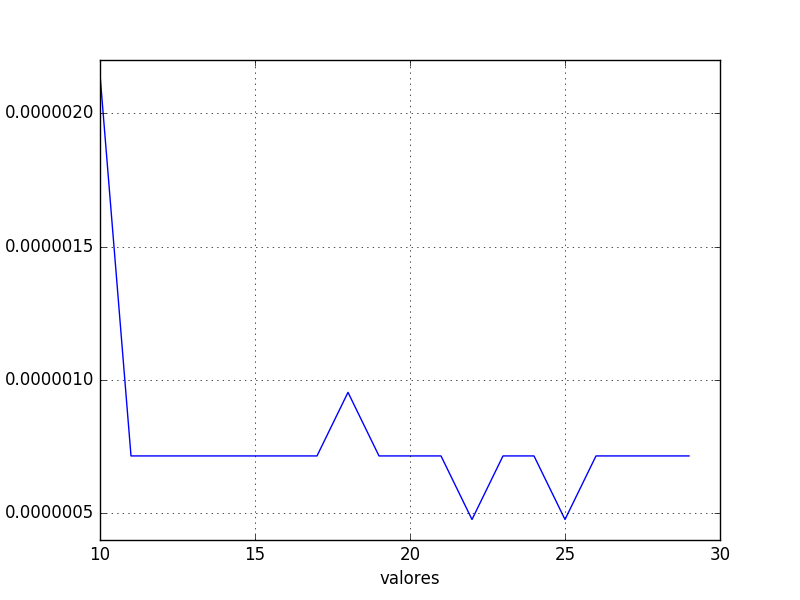
\includegraphics[width=.95\linewidth]{python_imgs/test_cache}
		  \caption{Implementação com cache}
		  \label{fig:sub1}
		\end{subfigure}%
		\begin{subfigure}{.5\textwidth}
		  \centering
		  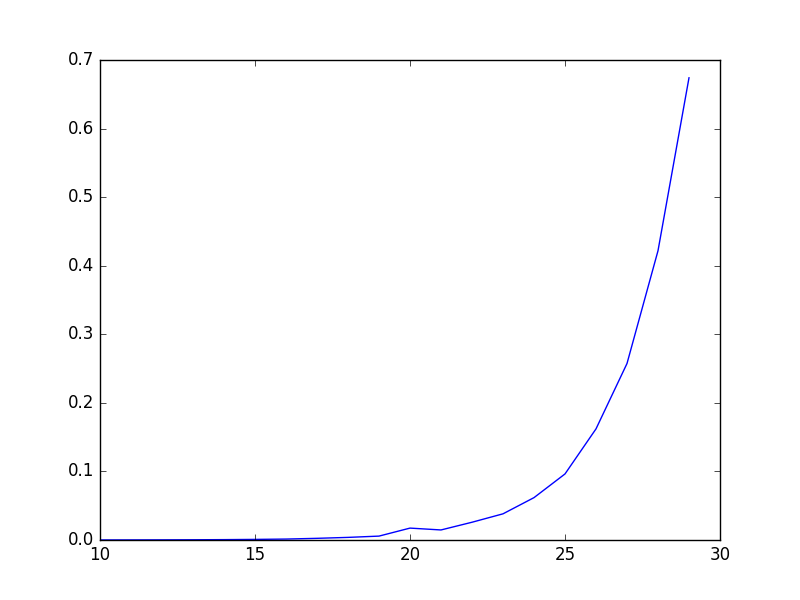
\includegraphics[width=.95\linewidth]{python_imgs/test_rec}
		  \caption{Implementação sem cache}
		  \label{fig:sub2}
		\end{subfigure}
		\caption{Tempos das implementações recursivas da função de Fibonacci com e sem cache}
		\label{fig:test}
	\end{figure}
\end{frame}

\subsection{Compilando programas em Python}

\begin{frame}[fragile]
	\frametitle{Compilando programs em Python}
	É necessário o módulo PyInstaller, disponível para Linux, Mac e Windows.

	\begin{lstlisting}
$ pip install PyInstaller
	\end{lstlisting}

	PyInstaller é...
\end{frame}

\begin{frame}[fragile]
	\frametitle{Compilando programs em Python}
	\lstinputlisting[style=scriptstyle]{python_scripts/python_compilado.py}
\end{frame}

\begin{frame}[fragile]
	\frametitle{Compilando programs em Python}

	\begin{lstlisting}
$ pyinstaller python_compilado.py
79 INFO: PyInstaller: 3.2
79 INFO: Python: 3.5.2
85 INFO: Platform: Linux-4.8.10-1-ARCH-x86_64-with-arch
85 INFO: wrote /home/gustavo/github/PythonPresentation/python_scripts/python_compilado.spec
87 INFO: UPX is not available.
93 INFO: Extending PYTHONPATH with paths
['/home/gustavo/github/PythonPresentation/python_scripts',
 '/home/gustavo/github/PythonPresentation/python_scripts']
93 INFO: checking Analysis
93 INFO: Building Analysis because out00-Analysis.toc is non existent
94 INFO: Initializing module dependency graph...
	\end{lstlisting}
\end{frame}

\begin{frame}[fragile]
	\frametitle{Compilando programs em Python}

	\begin{lstlisting}
$ cd dist
$ cd python_compilado
$ pwd
~/github/PythonPresentation/python_scripts/dist/python_compilado
$ ./python_compilado
Oi, tudo bem?
primeiro inteiro: 8
segundo inteiro: 9
17
	\end{lstlisting}
\end{frame}

%---------------------------------------------------------

\section{Aprenda Mais!}

\begin{frame}
	\frametitle{Aprenda Mais!}
	\begin{itemize}
		\item \textbf{Learning Python}. \textit{Mark Lutz}.O'Reilly.
		\item \textbf{Learning IPython for Interactive Computing and Data Visualization}.
\textit{Cyrille Rossant}. Packt Publishing Ltd. Birmingham, UK. 2015. ISBN 978-1-78398-698-9.
		\item \textbf{Mastering Pandas}. \textit{Femi Anthony}. Packt Publishing Ltd.
Birmingham, UK. 2015. ISBN 978-1-78398-196-0.
	\end{itemize}
\end{frame}

\begin{frame}
    Esta apresentação e todos os scripts apresentados estão disponíveis
no repositório no GitHub:
\url{https://github.com/gustavofsantos/PythonPresentation}
\end{frame}

\begin{frame}
\titlepage
\end{frame}

\end{document}
